Ce cycle désigne les principales étapes de développement du logiciel.
Le but de cette sécantation est de permettre la vérification du processus de déveeloppement.
Il comprend le plus souvent les étapes suivantes :
\begin{itemize}
        \item L'analyse des besoins et la faisabilité du projet
        \item La conception
        \item Le codage
        \item Les tests
        \item La documentation
        \item La mise en production
        \item La maintenance
\end{itemize}
Le cycle de vie peut être modélisé de plusieurs manières (Figures \ref{fig:methv}  et \ref{fig:methv2}).
Nous utiliserons ici le modèle du cycle en V car demeure actuellement le cycle de vie le 
plus connu et certainement le plus utilisé. 
Il s'agit d'un modèle en cascade dans lequel le 
développement des tests et du logiciel sont effectués 
de manière synchrone \cite{audibert2009uml}.

    \begin{figure}[t]
        \centering
        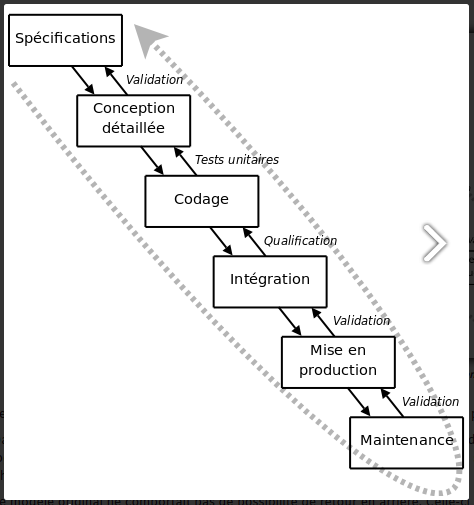
\includegraphics[scale=0.35]{images/Analyse_des_besoins/methcasc.png}
        \caption{Modèle du cycle de vie en cascade \cite{audibert2009uml}}
        \label{fig:methv}
    \end{figure}
    \begin{figure}[t]
        \centering
        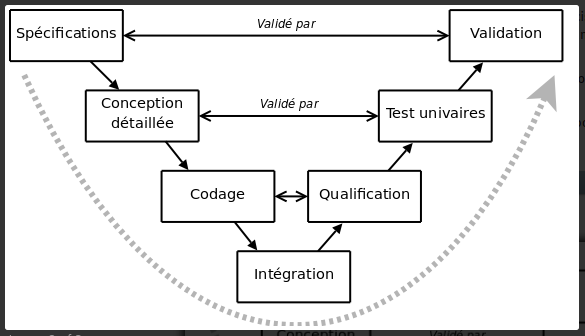
\includegraphics[scale=0.35]{images/Analyse_des_besoins/methv.png}
        \caption{Modèle du cycle de vie en V \cite{audibert2009uml}}
        \label{fig:methv2}
    \end{figure}